\setlength{\imagewidth}{80mm}%
\setlength{\imageheight}{\imagewidth}%
\DTLsetseparator{,}%
\DTLloaddb[noheader,keys={x,y,a}]{dbcorners}{figures/data/piecewise_smooth_surface/corners_xya.dat}%
\begin{tikzpicture}[%
	x=\imagewidth, y=\imageheight,
	img/.style={anchor=south west, inner sep=0}]
	%%% SURFACE
	\node[img] at (0,0) {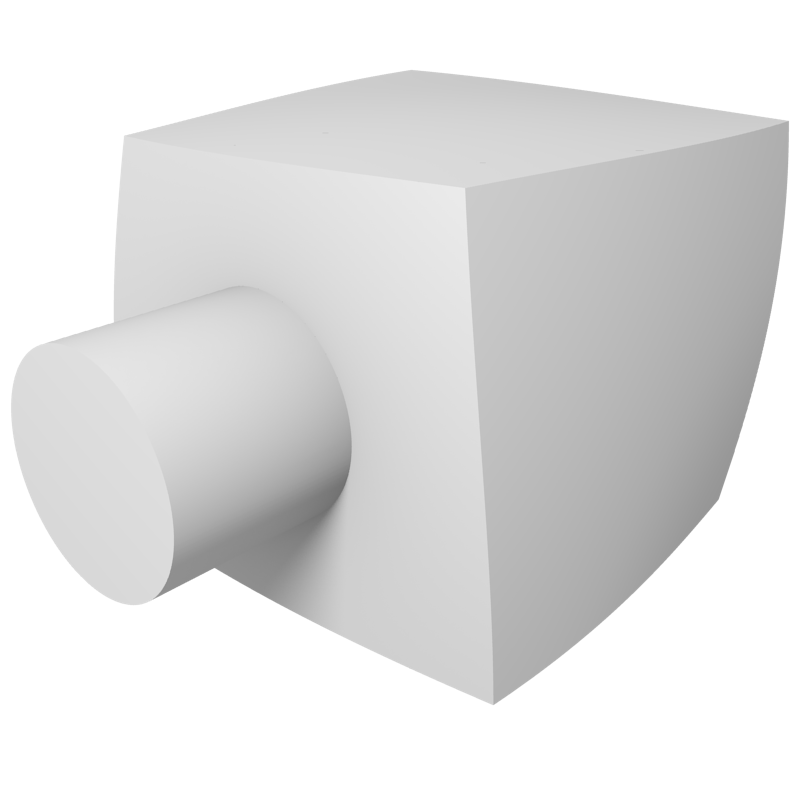
\includegraphics[width=\imagewidth]{piecewise_smooth_surface/surface}};
	%%% HIDDEN EDGES
	\node[img] at (0,0) {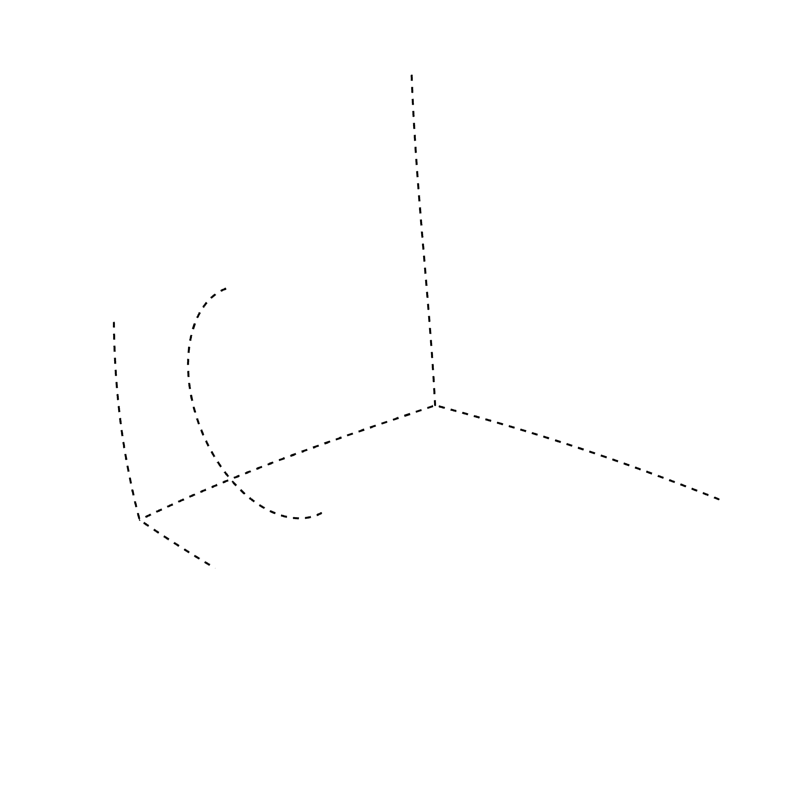
\includegraphics[width=\imagewidth]{piecewise_smooth_surface/edges_hidden}};
	%%% HIDDEN CORNERS
	\DTLforeach*{dbcorners}{\locx=x, \locy=y, \loca=a}{%
		\ifnum \loca = 0
			\fill[black] (\locx,\locy) circle (1.0pt);
		\fi
	}%
	%%% SURFACE (semi-transparent to mask hidden edges & corners)
	{\transparent{0.75}
		\node[img] at (0,0) {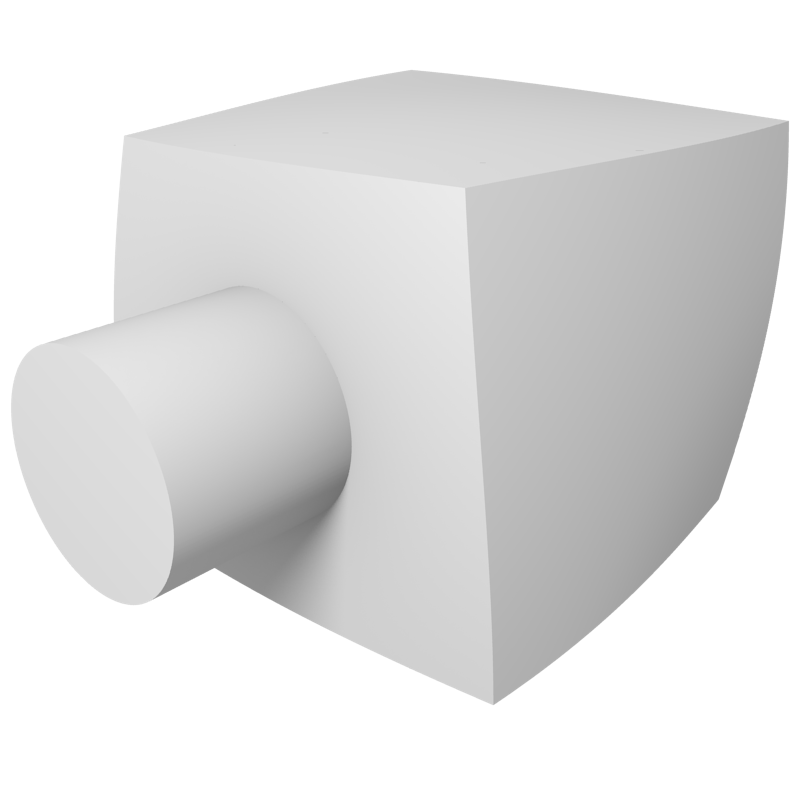
\includegraphics[width=\imagewidth]{piecewise_smooth_surface/surface}};
	}%
	%%% VISIBLE EDGES
	\node[img] at (0,0) {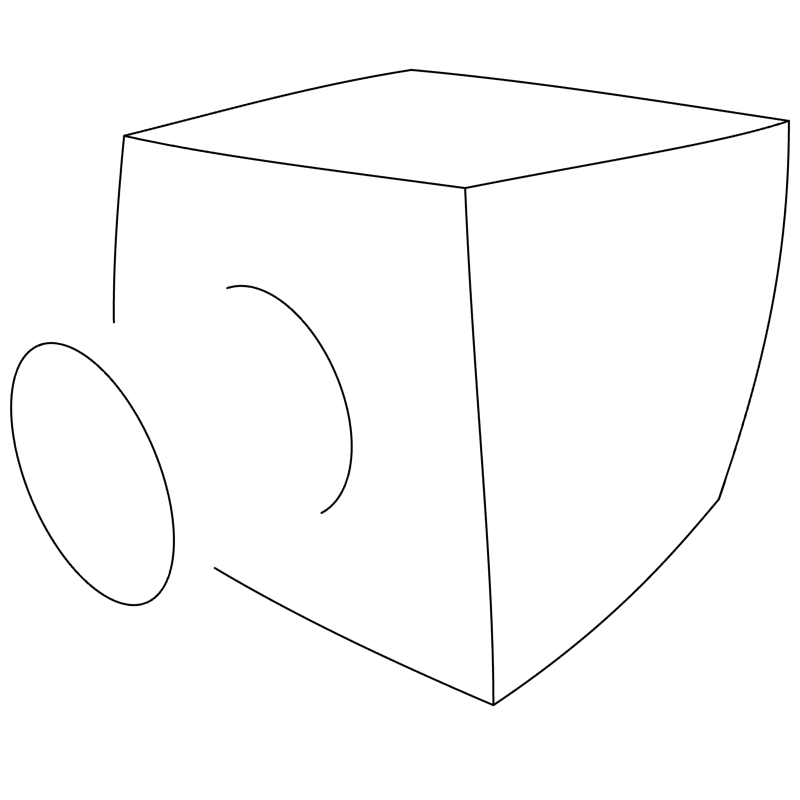
\includegraphics[width=\imagewidth]{piecewise_smooth_surface/edges_visible}};
	%%% VISIBLE CORNERS
	\DTLforeach*{dbcorners}{\locx=x, \locy=y, \loca=a}{%
		\ifnum \loca = 1
			\fill[black] (\locx,\locy) circle (1.0pt);
		\fi
	}%
	%
	%%% ANOTATIONS
	\DTLassign{dbcorners}{1}{\locxa=x,\locya=y,\loca=a}% 	
	\DTLassign{dbcorners}{4}{\locxb=x,\locyb=y,\loca=a}% 
	\DTLassign{dbcorners}{8}{\locxc=x,\locyc=y,\loca=a}% 
	\node[anchor=west] (anotIrrPts) at (\locxb,{0.5*(\locya + \locyb)}) {points irréguliers};
	\draw[shorten >=5pt, ->] (anotIrrPts.south) to [bend left=20] (\locxa, \locya);
	\draw[shorten >=5pt, ->] (anotIrrPts.north) to [bend right=20] (\locxb, \locyb);
	\draw[shorten >=5pt, ->] (anotIrrPts.west) to [bend left=10] (\locxc, \locyc);
\end{tikzpicture}
\DTLgdeletedb{dbcorners}%
